%% ------------------------------------------------------------------------- %%
\chapter{Evaluation}
\label{cap:experimentos}

In this section we present some experimental evaluations of the proposed extensions along with the original method in three widely known datasets: SFA, Pratheepan and HGR. In addition, a brief definition of the evaluation metrics used is shown for the sake of clarity.


%------------------------------------------------------
\section{Datasets}
\label{sec:datasets}

\subsection{UCI}
\label{sec:datasets_uci}
Named UCI in this work, this dataset was proposed by~\citet{uci-skin-dataset:12} and obtained from the machine learning repository of the University of California in Irvine \citep{lichman:13}. The dataset consists of images of various skin and non-skin textures obtained from thousands of arbitrary faces images of different ages, sex and races \citep{pal-texas:04, feret:96}.

The UCI contains 245,057 samples, composed of 3 attributes that constitute the input vector $x = [x_1, x_2, x_3]$, $x \in \mathbb{R}^{d}$, where $d$ is the space dimension which represents, respectively, blue (B), green (G) and red (R) channels of the RGB color model. In addition, a fourth column determines the class to which the sample $x$ belongs, denoted by $y$, where $y \in Y$ and $Y = \{+1, -1\}$. In other words, each sample is an RGB pixel with a given label.

The table~\ref{tbl:uci_dataset} exemplifies a short excerpt from the UCI database. It is worth mentioning that of the 245,057 samples, 194,198 are non-skin pixels and 50,859 pixels with different skin tones. In addition, the images that were used to extract the dataset were not made available by the authors.

\begin{table}[hb]
\centering
\begin{small}
\begin{tabular}{|c|c|c|c|} \hline
\thb{B} & \thb{G} & \thb{R}  & \thb{Label}  \\ \hline
74	    & 85      & 123	     & 1     \\
207	    & 215     & 255      & 1     \\
74      & 82      & 122	     & 1     \\
202     & 211     & 255      & 1     \\
54      & 72      & 125      & 1     \\
\ldots  &\ldots   & \dots    &\ldots \\
166     & 164     & 116      & -1    \\
148     & 150     & 91       & -1    \\
29      & 26      & 5        & -1    \\
167     & 166	  & 115	     & -1    \\
180	    & 177	  & 133	     & -1    \\ \hline
\end{tabular}
\caption[Excerpt with samples from the UCI dataset]{Excerpt with samples from the UCI dataset. Each of the first three columns represents a pixel channel of the RGB color space ranging from 0 to 255. The fourth column is the label assigned to the sample, which can assume +1 if it is skin and -1, otherwise. Originally, the class representing a non-skin pixel had value 2, replaced by -1 for compliance with the experiments.}
\label{tbl:uci_dataset}
\end{small}
\end{table}

Since the data are points in the RGB space, it is possible to plot it for a better interpretation of them, as shown in the figure~\ref{fig:dataset_uci}.

\begin{figure}[ht]
    \centering
    \begin{minipage}{0.45\textwidth}
        \includegraphics[width=\textwidth]{uci_skinns_plot}
    \end{minipage}
    ~ % space
    \begin{minipage}{0.45\textwidth}
        \includegraphics[width=\textwidth]{uci_skin_plot}
    \end{minipage}
    \caption[3-dimensional view of the RGB channels of the UCI dataset]{3-dimensional view of the RGB channels of the UCI dataset. The blue points are skin samples and the green ones are non-skin. On the left are all samples of the dataset; to the right only the skin samples. Source: proposed by the author.}
    \label{fig:dataset_uci}
\end{figure}


\subsection{SFA}
\label{sec:datasets_sfa}
SFA, the name of the dataset proposed by \citet{sfa-skin-dataset:13}, stands for Skin of FERET and AR Database. The SFA is a set of images of frontal faces obtained from two other color image databases: the FERET, created by~\citet{feret:96}, and the AR proposed by~\citet{ar-face-database:98}, which provided 876 and 242 images each, respectively. It is important to notice that AR images have a white background and small variations of skin color. In other words, the environment is more controlled than the images in FERET \cite{sfa-skin-dataset:13}. Figure~\ref{fig:sfa_dataset_exemplo} shows some of the 1,118 samples available.

\begin{figure}[ht]
    \centering
    \begin{subfigure}[t]{0.21\textwidth}
        \includegraphics[width=\textwidth]{sfa/ori/img4}
        \includegraphics[width=\textwidth]{sfa/gtc/img4}
        \includegraphics[width=\textwidth]{sfa/gt/img4}
    \end{subfigure}
    ~
    \begin{subfigure}[t]{0.21\textwidth}
        \includegraphics[width=\textwidth]{sfa/ori/img51}
        \includegraphics[width=\textwidth]{sfa/gtc/img51}
        \includegraphics[width=\textwidth]{sfa/gt/img51}
    \end{subfigure}
    ~
    \begin{subfigure}[t]{0.21\textwidth}
        \includegraphics[width=\textwidth]{sfa/ori/img112}
        \includegraphics[width=\textwidth]{sfa/gtc/img112}
        \includegraphics[width=\textwidth]{sfa/gt/img112}
    \end{subfigure}
    ~ % space
    \begin{subfigure}[t]{0.21\textwidth}
        \includegraphics[width=\textwidth]{sfa/ori/img14}
        \includegraphics[width=\textwidth]{sfa/gtc/img14}
        \includegraphics[width=\textwidth]{sfa/gt/img14}
    \end{subfigure}
    \caption[Examples of SFA face image database]{Examples of SFA face image database. First row are the original images and the second contain the colored ground truth with the skin color pixels annotated manually. The black color RGB = (0, 0, 0) was assigned to all pixels in the background. In the third row we have the binary ground truth images. We generated these samples based on the colored ground truth, by creating a mask, assigning (255, 255, 255) for the pixels which were not background (0, 0, 0). One can see some noise in the results, but the samples were enough for further experiments. In addition, the original images were not perfectly annotated. Therefore, some salt noise can be seen in non-skin regions. Source: \citet{sfa-skin-dataset:13}.}
    \label{fig:sfa_dataset_exemplo}
\end{figure}

\citet{sfa-skin-dataset:13} also extracted different window patches of each skin and non-skin samples to facilitate future research. The samples were randomly generated considering the ground truth mask \footnote{Ground truth is the term used to denote an image whose point of interest is properly segmented and highlighted, discarding the remaining pixels giving them uniform colors.} of each image, being three samples of skin and five of non-skin. Each sample is a window of size $n \times n$, where $n$ is odd, with a central pixel, from which other sample sizes have been created, ranging from $1 \times 1$ to $35 \times 35$, as can be seen in figure~\ref{fig:sfa_dataset_janelas}.

\begin{figure}[ht]
  \centering
  \includegraphics[width=.3\textwidth]{sfa-janelas}
  \caption[Structure of the windows that form the SFA samples]{Structure of the windows that form the SFA samples. In total, there are 3,354 skin samples and 5,590 non-skin samples for each window size. Source: \citet{sfa-skin-dataset:13}.}
  \label{fig:sfa_dataset_janelas}
\end{figure}

\textcolor{red}{Review} A partir das amostras criadas no SFA, um conjunto de dados foi extraído gerando uma base de dados de pele e não pele similar ao UCI na tabela~\ref{tbl:uci_dataset}. O tamanho da janela utilizado foi $9 \times 9$ e o espaço de cores também foi o RGB. Portanto, o total de amostras empregado nos experimentos é 724.464, sendo 271.674 de pele e 452.790 de não pele. A classe atribuída à cada amostra tem o mesmo valor que no UCI, ou seja, +1 se for pele e -1, caso contrário. A figura~\ref{fig:dataset_sfa} mostra a representação gráfica dos dados plotados em 3 dimensões.
\begin{figure}[hb]
    \centering
    \begin{minipage}{0.45\textwidth}
        \includegraphics[width=\textwidth]{sfa_skinns_plot}
    \end{minipage}
    ~ % space
    \begin{minipage}{0.45\textwidth}
        \includegraphics[width=\textwidth]{sfa_skin_plot}
    \end{minipage}
    \caption[Visão 3-dimensional dos canais RGB do conjunto de dados SFA]{\textcolor{red}{Review} Visão 3-dimensional dos canais RGB do conjunto de dados SFA. Os pontos em azul são amostras de pele e os verdes de não pele. À esquerda tem-se todas as amostras do conjunto de dados gerado; à direita apenas as amostras de pele. Fonte: proposto pelo autor.}
    \label{fig:dataset_sfa}
\end{figure}

\subsection{Pratheepan}
\label{sec:datasets_pratheepan}
The images in the Pratheepan dataset were downloaded randomly from Google for human skin detection search. There are 78 images of family and face captured with a range of distinct cameras using different color enhancement and under different illumination conditions \cite{tan:12}. Figure~\ref{fig:pra_dataset_exemplo} shows some of the 78 samples available.

\begin{figure}[hb]
    \centering
    \begin{subfigure}[t]{0.293\textwidth}
        \includegraphics[width=\textwidth]{pra/ori/07-c140-12family-red-rr-398h}
        \includegraphics[width=\textwidth]{pra/gt/07-c140-12family-red-rr-398h}
    \end{subfigure}
    ~
    \begin{subfigure}[t]{0.31\textwidth}
        \includegraphics[width=\textwidth]{pra/ori/3115267-My-very-large-Indian-family-2}
        \includegraphics[width=\textwidth]{pra/gt/3115267-My-very-large-Indian-family-2}
    \end{subfigure}
    ~
    \begin{subfigure}[t]{0.31\textwidth}
        \includegraphics[width=\textwidth]{pra/ori/buck_family}
        \includegraphics[width=\textwidth]{pra/gt/buck_family}
    \end{subfigure}
    \caption[Examples of Pratheepan skin dataset]{Examples of Pratheepan skin dataset. At the top is the original image and at the bottom the ground truth with the skin color pixels annotated. Here, the ground truth are binary images, where the black color RGB = (0, 0, 0) was assigned to all pixels in the background. Source: \citet{tan:12}.}
    \label{fig:pra_dataset_exemplo}
\end{figure}


\subsection{HGR}
\label{sec:datasets_hgr}
The database for Hand Gesture Recognition (HGR) contains the gestures from Polish and American Sign Language. There are 1,558 images acquired in different conditions of background, dimensions and lightening. In addition to original and ground truth binary skin mask images, it includes hand feature points location in separate files. Figure~\ref{fig:hgr_dataset_exemplo} shows some of the 1,558 samples available \citep{kawulok:14, nalepa:14, grzejszczak:16}.

The images within were acquired in three different series. A set of 899 was captured in uncontrolled background and lighting. A small set of 85 was obtained in gray (44) and (41) uncontrolled background; the lighting was uniform. The third group contains 574 images in controlled background (green tone), using uniform lighting conditions \citep{kawulok:14, nalepa:14, grzejszczak:16}.

\begin{figure}[hb]
    \centering
    \begin{subfigure}[t]{0.3\textwidth}
        \includegraphics[width=\textwidth]{hgr/ori/D_P_hgr1_id05_2}
        \includegraphics[width=\textwidth]{hgr/gt/D_P_hgr1_id05_2}
    \end{subfigure}
    ~
    \begin{subfigure}[t]{0.275\textwidth}
        \includegraphics[width=\textwidth]{hgr/ori/N_P_hgr1_id04_5}
        \includegraphics[width=\textwidth]{hgr/gt/N_P_hgr1_id04_5}
    \end{subfigure}
    ~
    \begin{subfigure}[t]{0.337\textwidth}
        \includegraphics[width=\textwidth]{hgr/ori/V_S_hgr2A2_id03_1}
        \includegraphics[width=\textwidth]{hgr/gt/V_S_hgr2A2_id03_1}
    \end{subfigure}
    \caption[Examples of HGR skin dataset]{Examples of HGR skin dataset. At the top is the original image and at the bottom the ground truth with the skin color pixels annotated. Differently from Pratheepan and SFA, the ground truth is also binary images, but the black color RGB = (0, 0, 0) was assigned to all pixels when they represent skin patches. Source: \citet{kawulok:14, nalepa:14, grzejszczak:16}.}
    \label{fig:hgr_dataset_exemplo}
\end{figure}


%------------------------------------------------------
\section{Primeiro experimento}
\label{sec:experimento_um}
O primeiro experimento foi realizado com $k$-NN e SVM, disponíveis no pacote \emph{scikit-learn} \citep{scikit-learn:11}. O espaço de cores usado originalmente foi o RGB, como citado na descrição dos conjuntos de dados em \ref{sec:datasets}. Em ambos os casos, a estratégia escolhida de validação cruzada foi a \emph{10-fold}, que é uma escolha comum desta abordagem na prática \citep{mostafa:12}. Além disso, a técnica de tabela de busca\index{busca!tabela de} do \emph{scikit-learn} também foi utilizada com o objetivo de encontrar os parâmetros mais adequados para cada classificador.

A tabela de busca é usada no \emph{scikit-learn} para encontrar os parâmetros ótimos de um classificador quando eles não podem ser aprendidos pelo estimador, tais como, \emph{kernel} e $\gamma$ na SVM ou número de vizinhos no $k$-NN \citep{scikit-learn:11}. As tabelas de parâmetros utilizadas no treinamento da SVM e $k$-NN podem ser vistas em \ref{tab:svm_tabela_busca} e \ref{tab:knn_tabela_busca}. Os parâmetros de cada linha são combinados na tentativa de encontrar o estimador ótimo. Por exemplo, uma escolha no treinamento da SVM seria \emph{kernel}=rbf, C=100, \emph{gamma}=1e-4. Todas as combinações possíveis são exploradas, sendo que a melhor delas é retornada \citep{scikit-learn:11}.

\begin{table}[!htpb]
\centering
\begin{small}
\setlength{\tabcolsep}{10pt}

\begin{tabular}{|c|c|c|c|c|c|c|c|c|c|}\hline
 \thbi{kernel} & \multicolumn{4}{c|}{\thbi{C}} & \multicolumn{3}{c|}{\thbi{gamma}} & \multicolumn{2}{c|}{\thbi{degree}}\\ \cline{1-10}
rbf    & 1 & 10 & 100 & 1000 & 1e-3 & 1e-4 & 1e-5 &   &   \\ \hline
poly   & 1 & 10 & 100 & 1000 &      & 1e-4 & 1e-5 & 3 & 4 \\ \hline
linear & 1 & 10 & 100 & 1000 &      &      &      &   &   \\ \hline

\end{tabular}
\end{small}
\caption[Tabela de busca dos parâmetros do estimador ótimo na SVM]{Tabela de busca dos parâmetros do estimador ótimo na SVM. A coluna kernel refere-se aos kernels usados no treinamento que são gaussiano, polinomial e linear, respectivamente. C é um parâmetro de regularização que diz à SVM a quantidade de erro admitido no treinamento. Gamma é um parâmetro usado somente nos kernels gaussiano e polinomial, conforme citado em \ref{sec:clasificadores_svm}. Degree é o grau do polinômio; usado somente no kernel polinomial \citep{scikit-learn:11}.}
\label{tab:svm_tabela_busca}
\end{table}

\begin{table}[!htpb]
\centering
\begin{small}
\setlength{\tabcolsep}{8pt}

\begin{tabular}{|c|c|c|c|c|c|c|c|c|c|c|c|c|}\hline
 \multicolumn{10}{|c|}{\thbi{n\_neighbors}} & \multicolumn{2}{c|}{\thbi{weights}} & \multicolumn{1}{c|}{\thbi{algorithm}}\\ \cline{1-13}
3 & 5 & 9 & 15 & 25 & 50 & 100 & 200 & 400 & 800 & distance & uniform & auto \\ \hline

\end{tabular} 
\end{small}
\caption[Tabela de busca dos parâmetros do estimador ótimo no $k$-NN]{Tabela de busca dos parâmetros do estimador ótimo no k-NN. A coluna n\_neighbors refere-se ao número de vizinhos considerado no treinamento. Weights é a função peso usada na predição, onde uniform indica que os pontos têm pesos iguais e distance indica que o inverso da distância é aplicado na classificação, conforme citado em \ref{eq:knn_funcao_peso}. A terceira coluna indica qual algoritmo deve ser utiizado; auto significa que o algoritmo será decidido com base nos dados \citep{scikit-learn:11}.}
\label{tab:knn_tabela_busca}
\end{table}

Os resultados deste experimento podem ser vistos na tabela \ref{tab:resultados_experimento_um}. Vale ressaltar que o treinamento foi executado com 10 tarefas em paralelo em ambos os classificadores e 30\% dos dados, aleatoriamente, foram separados para teste.
\begin{table}[!htpb]
\centering
\begin{small}
\setlength{\tabcolsep}{8pt}

\begin{tabular}{|c|c|c|c|c|c|}\hline
 \thb{Conjunto de dados} & \thb{Classificador} & \thb{Modelo de cores} & \thbi{Precision} & \thbi{Recall} & \thbi{F1-score} \\ \hline
 \multirow{2}{*}{UCI} & $k$-NN & RGB & 0,9995 & 0,9995 & 0,9995 \\ \cline{2-6}
                      & SVM    & RGB & 0,9995 & 0,9995 & 0,9995 \\ \hline
 \multirow{2}{*}{SFA} & $k$-NN & RGB & 0,9672 & 0,9669 & 0,9670 \\ \cline{2-6}
                      & SVM    & RGB & 0,9643 & 0,9628 & 0,9638 \\ \hline

\end{tabular}
\end{small}
\caption[Resultados dos experimentos com $k$-NN e SVM nos conjuntos de dados UCI e SFA]{Resultados dos experimentos com $k$-NN e SVM nos conjuntos de dados UCI e SFA. Os parâmetros ótimos do k-NN no treinamento com UCI foram n\_neighbors=3, weights=uniform e com SFA n\_neighbors=15, weights=uniform. Os parâmetros ótimos da SVM no treinamento com UCI e SFA foram kernel=rbf, C=100 e gamma=1e-3.}
\label{tab:resultados_experimento_um}
\end{table}

Como pode ser visto na tabela \ref{tab:resultados_experimento_um}, o $k$-NN teve resultados ligeiramente melhores que a SVM no conjunto de dados SFA. Ambos classificadores tiveram medidas de qualidade muito altas no conjunto de dados UCI, próximas a 100\%, o que, provavelmente, é uma situação de sobreajuste. Uma causa possível está na separação dos dados de treinamento e teste. Há muitas repetições entre as amostras, logo, é possível que amostras já vistas pelo classificador durante o treinamento sejam utilizadas na etapa de teste. Por essa razão, os experimentos subsequentes foram realizados somente com o SFA.

%------------------------------------------------------
\section{Segundo experimento}
\label{sec:experimento_dois}
Este experimento, de maneira similar ao realizado na seção \ref{sec:experimento_um}, também foi realizado com $k$-NN e SVM. Porém, o conjunto de dados SFA foi transformado para os espaços de cor HSV, Lab e YCbCr com o objetivo de compreender a influência nos resultados. Além disso, o atributo referente ao componente de luminância foi ignorado para que um teste somente com os componentes de crominância fosse realizado. Novamente, a estratégia escolhida de validação cruzada foi a \emph{10-fold}.

Como o objetivo deste experimento é avaliar a performance do classificador em espaços de cores distintos, os parâmetros ótimos obtidos no experimento \ref{sec:experimento_um} foram fixados aqui.

Os resultados podem ser vistos na tabela \ref{tab:resultados_experimento_dois}. Vale ressaltar que o treinamento foi executado com 10 tarefas em paralelo em ambos os classificadores e 30\% dos dados, aleatoriamente, foram separados para teste.
\begin{table}[!htpb]
\centering
\begin{small}
\setlength{\tabcolsep}{8pt}

\begin{tabular}{|c|c|c|c|c|}\hline
 Modelo de cores & Classificador & \emph{Precision} & \emph{Recall} & \emph{F1-score} \\ \hline
 \multirow{2}{*}{RGB}   & $k$-NN  & 0,9672 & 0,9669 & 0,9670 \\ \cline{2-5}
                        & SVM     & 0,9643 & 0,9628 & 0,9638 \\ \hline
 \multirow{2}{*}{HSV}   & $k$-NN  & 0,9676 & 0,9673 & 0,9674 \\ \cline{2-5}
                        & SVM     & 0,9718 & 0,9677 & 0,9679 \\ \hline
 \multirow{2}{*}{HS}    & $k$-NN  & 0,9215 & 0,9194 & 0,9199 \\ \cline{2-5}
                        & SVM     & 0,9305 & 0,9302 & 0,9302 \\ \hline
 \multirow{2}{*}{Lab}   & $k$-NN  & 0,9671 & 0,9660 & 0,9670 \\ \cline{2-5}
                        & SVM     & 0,9675 & 0,9665 & 0,9672 \\ \hline
 \multirow{2}{*}{ab}    & $k$-NN  & 0,9444 & 0,9439 & 0,9440 \\ \cline{2-5}
                        & SVM     & 0,9451 & 0,9447 & 0,9446 \\ \hline
 \multirow{2}{*}{YCbCr} & $k$-NN  & 0,9679 & 0,9677 & 0,9677 \\ \cline{2-5}
                        & SVM     & 0,9635 & 0,9633 & 0,9632 \\ \hline
 \multirow{2}{*}{CbCr}  & $k$-NN  & 0,9487 & 0,9482 & 0,9483 \\ \cline{2-5}
                        & SVM     & 0,9496 & 0,9492 & 0,9493 \\ \hline

\end{tabular}
\end{small}
\caption[Resultados dos experimentos com $k$-NN e SVM no conjunto de dados SFA em espaços de cores distintos]{Resultados dos experimentos com $k$-NN e SVM no conjunto de dados SFA em espaços de cores distintos. As linhas com os modelos de cores HS, ab e CbCr indicam que o componente de luminância não foi utilizado no treinamento.}
\label{tab:resultados_experimento_dois}
\end{table}

Os melhores resultados com a SVM e $k$-NN foram obtidos nos espaços de cores HSV e YCbCr, respectivamente. Dentre aqueles onde o componente de luminância foi ignorado, o CbCr teve a melhor performance.

É interessante observar que os indicadores de qualidade do modelo mostram que ambos classificadores tiveram taxas ao redor de 96\% em todos os espaços de cor, quando aplicado com os 3 canais. Além disso, quando o canal de luminância foi ignorado, o desempenho foi inferior - aproximadamente 4 pontos percentuais no pior caso. Por outro lado, a perda de performance pode ser compensada pela redução da complexidade do modelo, já que uma dimensão pode ser descartada, mantendo, ainda, medidas de qualidade relativamente significativas.